\section{Durchführung}
\label{sec:Durchführung}


Zwei Stäbe mit unterschiedlicher Legierung werden nacheinader wie in Abiildung 6 einseitig eingespannt.

\begin{figure}[H]
  \centering
  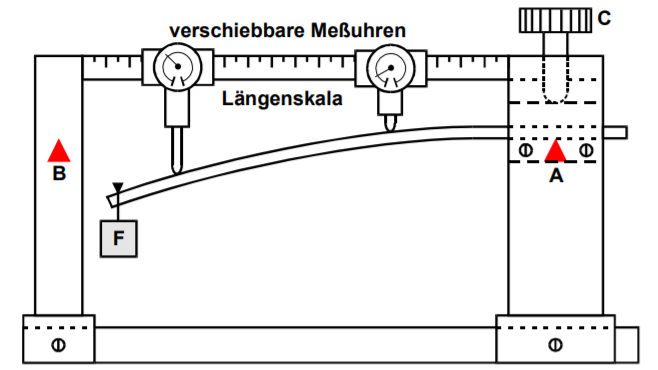
\includegraphics[height=5cm]{einseitig.PNG}
  \caption{Messapparatur für einen einseitig eingespannten Stab}
  \label{fig:einseitig}
\end{figure}

In $2$cm Abständen wird die Durchbiegung, jeweils mit einem an dem Stab hängendem Gewicht
und ohne einem gemessen. Diese Prozedur wird mit zwei Stäben durchgeführt.

Ein dritter Stab wird in dem Punkt A, wie in Abbildung 6 zusehen, eingespannt und
in Punkt B aufgelegt. Es wird analog wie bei den anderen Stäben vorgegangen links
und rechts des Gewichtes die Durchbiegung gemesen.

Zudem werden die Massen der Stäbe und Gewichte mit einer Waage ermittelt. Die Maße der
Stäbe werden mit einem Maßband und einer Schieblehre gemessen.
